\documentclass[a4paper, 12pt, notitlepage]{report}

%%%%%%%%%%%%%%%%%%%%%%%%%%%%%%%%%%%%%%%%%%%%%%%%%%%%%%
% Report template for latex
%%%%%%%%%%%%%%%%%%%%%%%%%%%%%%%%%%%%%%%%%%%%%%%%%%%%%%
% author: Ashok Fernandez <ashok.fernandez@gmail.com>
% date: 01-05-2013
% licence: This content is released under the (http://opensource.org/licenses/MIT) MIT License.
%%%%%%%%%%%%%%%%%%%%%%%%%%%%%%%%%%%%%%%%%%%%%%%%%%%%%%

% Comment to remove 'DRAFT' watermark
%\usepackage{draftwatermark}

%%%%%%%%%%%%%%%%%%%%%%%%%%%%%%%%%%%%%%%%%%%%%%%%%%%%%%
%%%%%%%%%%%%%%%%%%%%%%%%%%%%%%%%%%%% DOCUMENT SETTINGS
% Notes:    Comment out any packges you want to remove
%%%%%%%%%%%%%%%%%%%%%%%%%%%%%%%%%%%%%%%%%%%%%%%%%%%%%%

% If you want blackboard bold symbols e.g. for real numbers
\usepackage{amsfonts} 

% If you want to include jpeg or pdf pictures
\usepackage{graphicx} 

% Lets you use \url{} to create clickable hyperlinks
\usepackage{hyperref}

% Helvetica Font
\renewcommand{\familydefault}{\sfdefault} 
\usepackage{helvet}

% Wraps text around figures
\usepackage{wrapfig} 

% Let you include PDFs
% e.g \includepdf[pages={1,3,5}]{myfile.pdf}
\usepackage{pdfpages}

% Set bibliography engine as biblatex
\usepackage[backend=bibtex,
style=numeric
%style=alphabetic
%style=reading
]{biblatex}
\addbibresource{references}

% Reduce the margins of the page
\usepackage[margin=0.7in]{geometry} 

% Allows the title formats to be modified
\usepackage{titlesec} 

%%%%%%%%%%%%%%%%%%%%%%%%%%%%%%%%%%%%%%%%%%%%%%%%%%%%%%
%%%%%%%%%%%%%%%%%%%%%%%%%%%%%%%%% PRELIMINARY MATERIAL
%%%%%%%%%%%%%%%%%%%%%%%%%%%%%%%%%%%%%%%%%%%%%%%%%%%%%%

\begin{document}

% Title
\title{\LaTeX\ Report Template} 
\author{Ashok Fernandez} 
\date{\today} 

\maketitle

% Add the table of contents
\tableofcontents 

% Makes the chapter headers not say 'Chapter 1'
\titleformat{\chapter}[display]
 {\normalfont\huge\bfseries}{}{1em}{}

% Alters the space before and after the title
\titlespacing*{\chapter}{0pt}{-5em}{30pt}

% Line spacing for the remainder of the document
\setlength{\parskip}{0.8em}



%%%%%%%%%%%%%%%%%%%%%%%%%%%%%%%%%%%%%%%%%%%%%%%%%%%%%%
%%%%%%%%%%%%%%%%%%%%%%%%%%%%%%%%%%%%%%%%%%%% MAIN TEXT
%%%%%%%%%%%%%%%%%%%%%%%%%%%%%%%%%%%%%%%%%%%%%%%%%%%%%%





% Example of footnotes, plain text (will not be processed in case you want to use special charaters) and linking URLs
\chapter{How to make a document that looks good}
This document is an example of how to use \LaTeX, a mean little program which lets you worry about writing good content and not about laying it out. Here is some \texttt{plain ass text} \footnote{This confirms that that text was pretty damn plain - \url{www.shitty-text.com}}. 

\section{Look how this text wraps around the figure!}
A puppy is a juvenile dog. Some puppies may weigh 1–3 lb (0.45–1.4 kg), while larger ones can weigh up to 15–23 lb (6.8–10 kg). All healthy puppies grow quickly after birth. A puppy's coat color may change as the puppy grows older, as is commonly seen in breeds such as the Yorkshire Terrier. In vernacular English, puppy refers specifically to dogs while pup may often be used for other mammals such as seals, giraffes, guinea pigs, or even rats.

% Picture of a puppy! - Let's break it down
% This inserts a container for the picture that is 30% the width of the page
% The 'R' specifies its on the right of the page
\begin{wrapfigure}{RH}{0.30\textwidth} 
    
    % If you add a \label in your text you can refer to it later e.g
    % "Figure \ref{fig:puppy} demonstrates the common house puppy on a tree"
    \label{fig:puppy}
    
    % This will center the image in the middle of the container
    \begin{center} 
    
        % vspace adds vertical whitespace, this can be negative to shift a picture up
        \vspace{-25px} 
        
        % Make the picture 23% of the page width so it doesn't over-run the container
        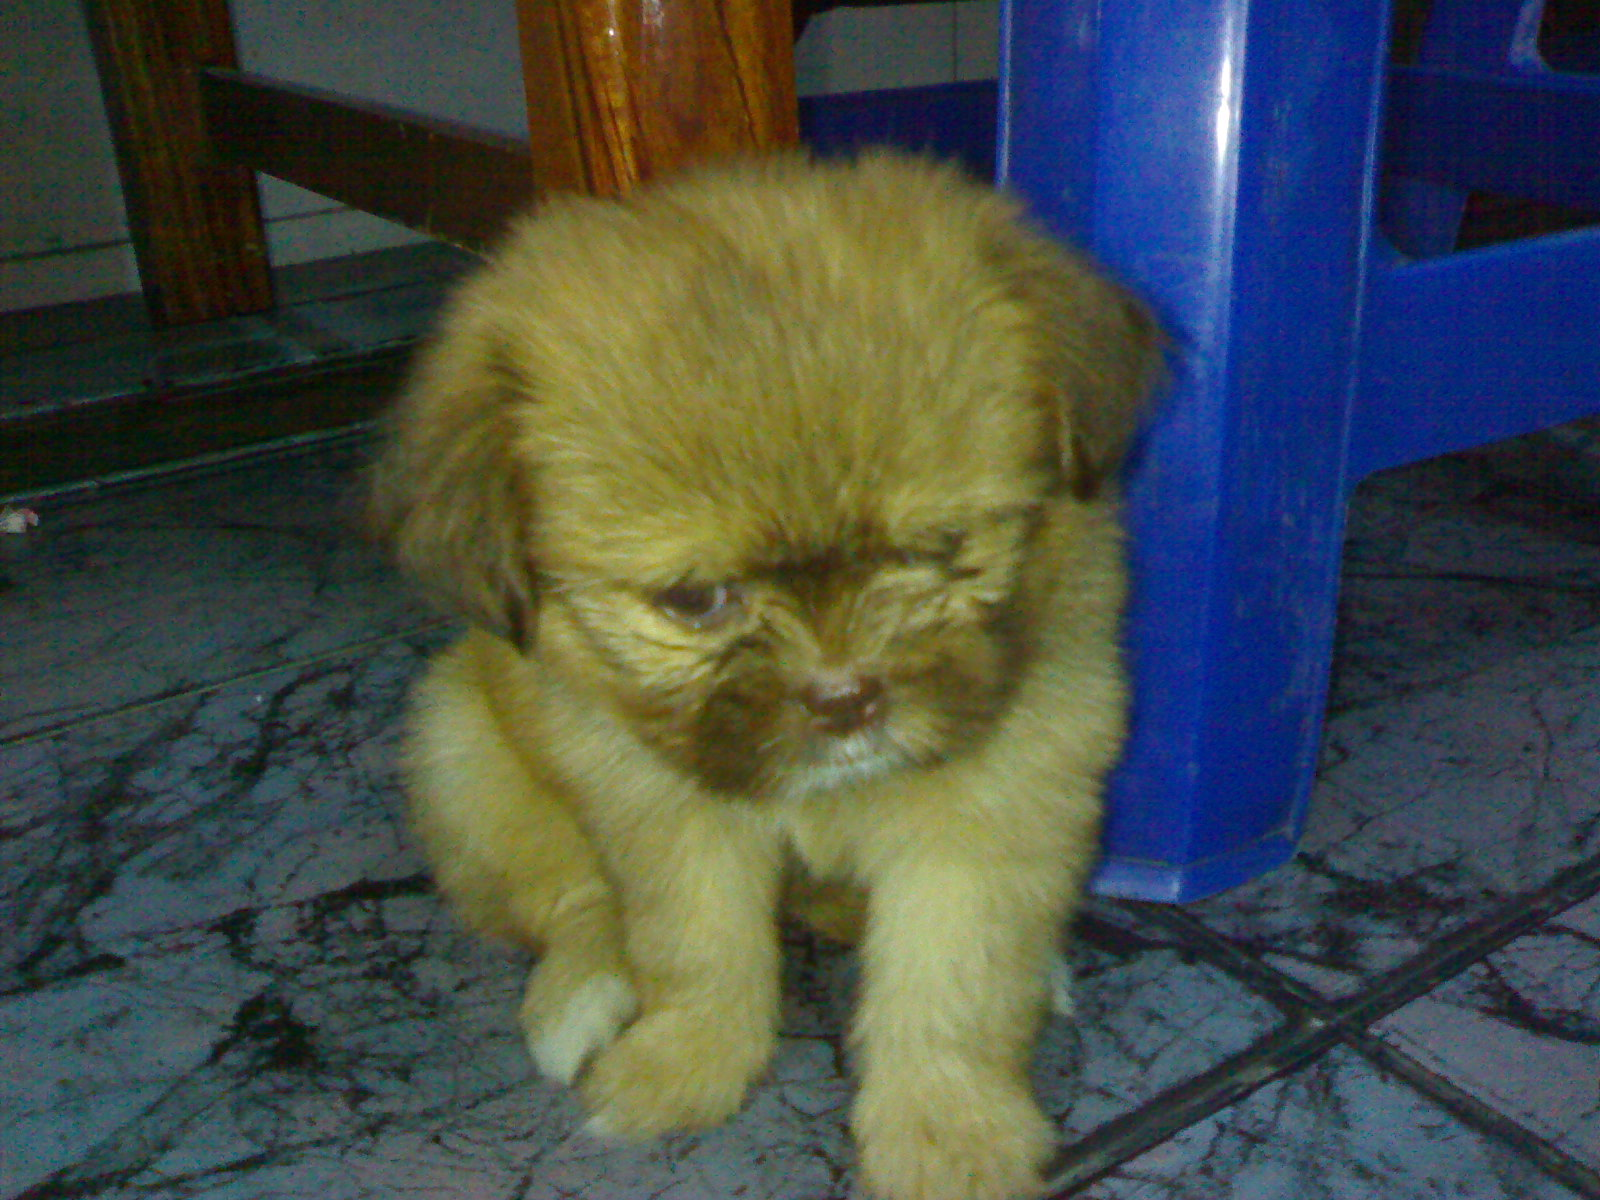
\includegraphics[width=0.28\textwidth]{images/puppy.jpg}
        
    \end{center}
  
    % Add a caption, remove \small if you want bigger text
    \caption{\small Puppy chilling}
    
    % This vspace will allow the text to wrap tighter below the caption
    \vspace{-10px}

\end{wrapfigure}


Born after an average of 63 days of gestation, puppies emerge in an amnion that is bitten off and eaten by the mother dog. Puppies begin to nurse almost immediately. If the litter exceeds six puppies, particularly if one or more are obvious runts, human intervention in hand-feeding the stronger puppies is necessary to ensure that the runts get proper nourishment and attention from the mother. As they reach one month of age, puppies are gradually weaned and begin to eat solid food. The mother may regurgitate partially digested food for the puppies or might let them eat some of her solid food. The mother dog usually refuses to nurse at this stage, though she might let them occasionally nurse for comfort. At first, puppies spend the large majority of their time sleeping and the rest feeding. They instinctively pile together into a heap, and become distressed if separated from physical contact with their littermates, by even a short distance.




% Example of using citations (see references.bib for citation source)
\section{Citations}
Two items are cited: \textit{The \LaTeX\ Companion} book \cite{latexcompanion} and the Donald Knuth's website \cite{knuthwebsite}. 

% Example of cross-referencing back to stuff thats in your document
\subsection{Related Citations in A Subsection}
Refering to figure \ref{fig:puppy}... oh look a RELATED CITATION \cite{latexcompanion,knuthwebsite}. 

% Print the bibliography
\printbibliography

\end{document}
